% HFUT_Courge_Project
\documentclass[UTF8]{ctexart}
\usepackage{fancyhdr}
\usepackage{graphicx}
\usepackage{titlesec}
\usepackage{titletoc}
\usepackage{listings}
\usepackage{appendix}
\usepackage{bm, amsmath,amsfonts}
\usepackage{multirow}
\usepackage[a4paper,left=3.4cm,right=3cm,top=1.65cm,bottom=2.54cm]{geometry}
\renewcommand{\contentsname}{\zihao{3} 目\quad 录}
\renewcommand{\abstractname}{\zihao{3} 摘\quad 要}
%页眉页脚设置
\pagestyle{fancy}
\fancyhf{}
\cfoot{\thepage}
%\rhead{\kaishu~XX课程设计~}

%目录页设置
\titlecontents{section}[0em]{\zihao{4}\bf }{\thecontentslabel\ }{}
{\hspace{.5em}\titlerule*[4pt]{$\cdot$}\contentspage}
\titlecontents{subsection}[2em]{\vspace{0.1\baselineskip}\zihao{-4}}{\thecontentslabel\ }{}
{\hspace{.5em}\titlerule*[4pt]{$\cdot$}\contentspage}
\titlecontents{subsubsection}[4em]{\vspace{0.1\baselineskip}\zihao{-4}}{\thecontentslabel\ }{}
{\hspace{.5em}\titlerule*[4pt]{$\cdot$}\contentspage}
%代码设置
\RequirePackage{listings}
\RequirePackage{xcolor}
\definecolor{dkgreen}{rgb}{0,0.6,0}
\definecolor{gray}{rgb}{0.5,0.5,0.5}
\definecolor{mauve}{rgb}{0.58,0,0.82}
\lstset{
	numbers=left,  
	frame=tb,
	aboveskip=3mm,
	belowskip=3mm,
	showstringspaces=false,
	columns=flexible,
	framerule=1pt,
	rulecolor=\color{gray!35},
	backgroundcolor=\color{gray!5},
	basicstyle={\ttfamily},
	numberstyle=\tiny\color{gray},
	keywordstyle=\color{blue},
	commentstyle=\color{dkgreen},
	stringstyle=\color{mauve},
	breaklines=true,
	breakatwhitespace=true,
	tabsize=3,
}
%------------------------------------------------------------------------
%正文部分
\begin{document}
	\begin{titlepage}
               	
\includegraphics[width=3.0cm,height=3.0cm]{gdut1.jpg}\\

		%\vspace*{1.5cm}
		\centering
		\quad
\includegraphics[width=13cm,height=4cm]{gdut.jpg}\\
		\vspace*{0.5cm}
		{\fontsize{30pt}\baselineskip 现\quad\ 代\quad\ 控\quad\ 制\quad\ 理\quad\ 论\quad\ 基\quad\ 础}\\

		 \vskip 2.0cm
		 \fontsize{19pt}\baselineskip
		 \makebox[30mm]{题目名称}
		 \underline{\makebox[75mm][c]{  实验报告}}\\%在这里修改成自己的题目
		 \vskip 0.9cm
		 \makebox[30mm]{学生姓名}
		 \underline{\makebox[75mm][c]{ xxx}}\\
		 \vskip 0.9cm
		 \makebox[30mm]{学\qquad\qquad 号}
		 \underline{\makebox[75mm][c]{ \LARGE12345678}}\\
		 \vskip 0.9cm
		 \makebox[30mm]{专业班级}
		 \underline{\makebox[75mm][c]{ xxxxx}}\\
		 \vskip 0.9cm
		  \makebox[30mm]{指导教师}
		 \underline{\makebox[75mm][c]{ xxx}}\\
		 \vskip 2cm
		 \LARGE \textbf{\number \year }~年~\textbf{\number\month}~月~\textbf{\number\day}~日		 
	\end{titlepage}



\tableofcontents\thispagestyle{empty}
\newpage
\setcounter{page}{1}
\section{实验一 \quad 系统的传递函数阵和状态空间表达式的转换 }

\subsection{ 实验目的 }
\par 1.学习多变量系统状态空间表达式的建立方法、了解系统状态空间表达式与传递函数相互转换的方法; 
\par 2.通过编程、上机调试,掌握多变量系统状态空间表达式与传递函数相互转换方法。
\subsection{实验内容 }
\par 1.系统的模型表达式如下:
\begin{equation}
   \left  \{\begin{aligned}
      \dot x=Ax+Bu    \\
      y=Cx+D     \\
        \end{aligned}\\
        x\in{R^{n}},u\in{R^{m}},y\in{R^{p}}\\
    \right.
 \end{equation}
 
\par 其中A为n×n维系数矩阵、B为n×m维输入矩阵、C为p×n维输出矩阵,D为传递阵,一般情况下为 0,只有n和m维数相同时,D=1。系统的传递函数阵和状态空间表达式之间的关系如式(2)所示。
\begin{equation}
G(s)= \frac {num(s)}{den(s)}=C(SI-A)^{-1}B+D
\end{equation}

\par 其中num(s)表示传递函数阵的分子阵,其维数是 p×m;den(s)表示传递函数阵的按s降幂排列的分母。

\par 2.实验步骤
\par(1)已知 SISO 系统的状态空间表达式如下:
\begin{equation}
    \begin{bmatrix}
    \dot x_1\\
    \dot x_2\\
    \dot x_3\\
    \end{bmatrix}=\begin{bmatrix}
    0 & 1 & 0\\
    0 & 0 & 1\\
    -4 & -3 & -2\end{bmatrix}\begin{bmatrix}
    x_1\\
    x_2\\
    x_3\\
    \end{bmatrix}+\begin{bmatrix}
    1\\
    3\\
    -6\\
    \end{bmatrix}u  , \quad   y=\begin{bmatrix}
    1 & 0 & 0 \\
    \end{bmatrix}\begin{bmatrix}
    x_1\\
    x_2\\
    x_3\\
    \end{bmatrix}
\end{equation}

\par 求系统的传递函数matlab程序如下:
\par  \begin{lstlisting}[language=matlab,escapeinside=``]
clear all
close all
clc

A=[0 1 0;0 0 1;-4 -3 -2];
B=[1;3;-6];
C=[1 0 0];
D=0;
[num,den]=ss2tf(A,B,C,D,1);
\end{lstlisting}

\par 程序运行结果:
\par  \begin{lstlisting}[language=matlab,escapeinside=``]
num =
         0    1.0000    5.0000    3.0000
den =
    1.0000    2.0000    3.0000    4.0000
\end{lstlisting}

\par 从程序运行结果可得到系统的传递函数为:
\par  \begin{lstlisting}[language=matlab,escapeinside=``]
G(s) =
      s^2 + 5 s + 3
  ---------------------
  s^3 + 2 s^2 + 3 s + 4
\end{lstlisting}

\par (2)从系统的传递函数(4)式求状态空间表达式的程序如下:
\par  \begin{lstlisting}[language=matlab,escapeinside=``]
num=[0 1 5 3];
den=[1 2 3 4];
[A,B,C,D]=tf2ss(num,den)
G_s=tf(num,den)
\end{lstlisting}

\par 程序的运行结果
\par  \begin{lstlisting}[language=matlab,escapeinside=``]
A =
    -2    -3    -4
     1     0     0
     0     1     0
B =
     1
     0
     0
C =
     1     5     3
D =
     0   
G_s =
      s^2 + 5 s + 3
  ---------------------
  s^3 + 2 s^2 + 3 s + 4
\end{lstlisting}
\par (3)对上述结果进行验证,matlab程序如下:
\par  \begin{lstlisting}[language=matlab,escapeinside=``]
A=[-2 -3 -4;1 0 0;0 1 0];
B=[1;0;0];
C=[1 5 3];
D=0;
[num,den]=ss2tf(A,B,C,D,1)
G_s=tf(num,den)
\end{lstlisting}
\par 程序的运行结果
\par  \begin{lstlisting}[language=matlab,escapeinside=``]
num =
     0     1     5     3
den =
    1.0000    2.0000    3.0000    4.0000
G_s =
      s^2 + 5 s + 3
  ---------------------
  s^3 + 2 s^2 + 3 s + 4
\end{lstlisting}
\par 程序运行结果与(2)相同。
\subsection{ 实验报告要求 }
\par 在运行以上[例]程序的基础上,应用 MATLAB 对(5)系统仿照[例 1.2]编程,求系统的A、B、C、阵;然后再仿照[例 1.3]进行验证
\begin{equation}
G(s)= \frac {\begin{bmatrix}s+2\\s^{2}+5s+3\\\end{bmatrix}}{s^{3}+2s^{2}+3s+4} \\
\end{equation}
\par Matlab程序如下:
\par  \begin{lstlisting}[language=matlab,escapeinside=``]
% %% 实验1应用
num=[0 0 1 2;0 1 5 3];
den=[1 2 3 4];
[A,B,C,D]=tf2ss(num,den)
%验证
A=[-2 -3 -4;1 0 0;0 1 0];
B=[1;0;0];
C=[0 1 2;1 5 3];
D=[0;0];
[num,den]=ss2tf(A,B,C,D,1)
\end{lstlisting}
\par 程序的运行结果
\par  \begin{lstlisting}[language=matlab,escapeinside=``]
A =
    -2    -3    -4
     1     0     0
     0     1     0
B =
     1
     0
     0
C =
     0     1     2
     1     5     3
D =
     0
     0
num =
     0     0     1     2
     0     1     5     3
den =
    1.0000    2.0000    3.0000    4.0000
\end{lstlisting}
\par 结果符合
\subsection{ 讨论 }
\par 系统传递函数模型和状态空间描述之间的区别和联系。
\par (1)传递函数表征其中直接或间接地由输入可控制和从输出中可观测到的那一部分,对于系统内部结构是不便描述的
\par(2)状态空间描述能反映系统全部独立变量的变化,从而能同时确定系统的全部内部运动状态。

\newpage
\section{实验二 \quad 状态空间控制模型系统仿真及状态方程求解 }
\subsection{ 实验目的 }
\par 1.熟悉线性连续系统的状态空间控制模型的各种表示方法 
\par 2.熟悉系统模型之间的转换功能
\par 3.利用 MATLAB 对线性定常系统进行动态分析
\subsection{实验内容 }
\par 1.系统的模型表达式如下:
\begin{equation}
G(s)= \frac{s^{3}+2s^{2}+s+3}{s^{3}+0.5s^{2}+2s+1}
 \end{equation}
 
\par 求上式系统的零极点增益模型和状态空间模型,并求其单位脉冲响应及单位阶跃响应
\par Matlab程序如下:
\par  \begin{lstlisting}[language=matlab,escapeinside=``]
num=[1 2 1 3];
den=[1 0.5 2 1];
sys=tf(num,den);
sys1=tf2zp(num,den);
sys2=tf2ss(num,den);
figure(1)
impulse(sys);
axis([0 35 -1 1.5])
grid on
figure(2)
step(sys);
axis([0 35 0 4])
grid on

sys=tf(num,den)
sys1=tf2zp(num,den)
[a,b,c,d]=tf2ss(num,den)
\end{lstlisting}

\par 运行结果如下:
\par  \begin{lstlisting}[language=matlab,escapeinside=``]
sys =
    s^3 + 2 s^2 + s + 3
  -----------------------
  s^3 + 0.5 s^2 + 2 s + 1

sys1 =
  -2.1746 + 0.0000i
   0.0873 + 1.1713i
   0.0873 - 1.1713i
a =
   -0.5000   -2.0000   -1.0000
    1.0000         0         0
         0    1.0000         0
b =
     1
     0
     0
c =
    1.5000   -1.0000    2.0000
d =
     1
\end{lstlisting}

\par \begin{figure} [h]  
\begin{minipage}[t]{0.5\linewidth}  
\centering  
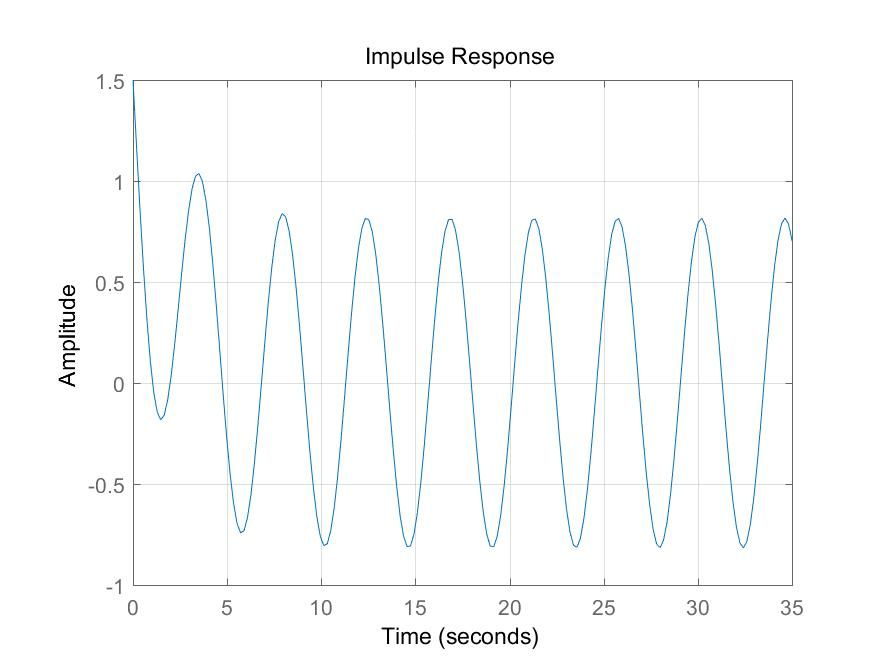
\includegraphics[width=2.8in]{fig/2-1.jpg}  
\caption{单位脉冲响应}  
\label{fig:side:a}  
\end{minipage}%  
\begin{minipage}[t]{0.5\linewidth}  
\centering  
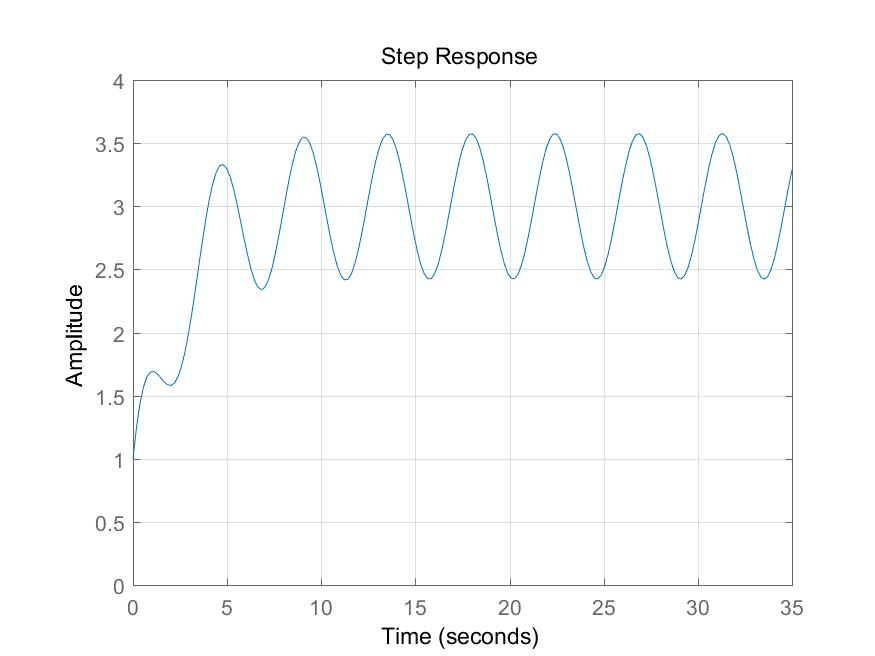
\includegraphics[width=2.8in]{fig/2-2.jpg}  
\caption{单位阶跃响应}  
\label{fig:side:b}  
\end{minipage}  
\end{figure} 

\par 2.考虑由以下状态方程描述的系统
\begin{equation}
    \begin{bmatrix}
    \dot x_1\\
    \dot x_2\\
    \end{bmatrix}=\begin{bmatrix}
    0 & 1 \\
    -10 & -5 \\ \end{bmatrix}\begin{bmatrix}
    x_1\\
    x_2\\
    \end{bmatrix} ,  \quad \begin{bmatrix}
    x_1(0)\\
    x_2(0)\\
    \end{bmatrix}=\begin{bmatrix}
    2  \\
    1  \\
    \end{bmatrix}  ,  \quad  \begin{bmatrix}
    y_1\\
    y_2\\
    \end{bmatrix}=\begin{bmatrix}
    1 & 0 \\
    0 & 1 \\ \end{bmatrix}\begin{bmatrix}
    x_1\\
    x_2\\
    \end{bmatrix}
\end{equation}
\par 求该系统状态对初始状态的时间响应

\par Matlab程序如下:
\par  \begin{lstlisting}[language=matlab,escapeinside=``]
A=[0 1;-10 -5];
B=[0;0];
D=B;
C=[1 0;0 1];
x0=[2;1];
[y,x,t]=initial(A,B,C,D,x0);
figure(3)
plot(t,x(:,1),t,x(:,2))
grid on
title('Response to Initial Condition')
xlabel('Time(sec)')
ylabel('x1,x2');
text(0.55,1.15,'x1')
text(0.4,-2.9,'x2')
legend('x1','x2')
\end{lstlisting}

\par 运行结果如下:
\par \begin{figure}[h]       
 \center{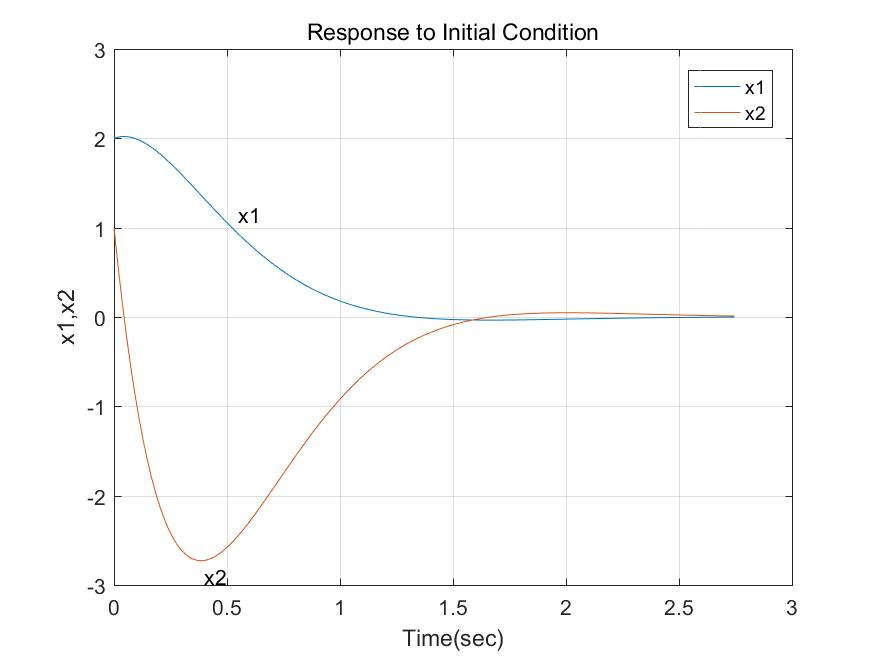
\includegraphics[width=8cm]  {fig/2-3.jpg}}      
 \caption{\label{1} 系统状态对初始条件的响应曲线} 
 \end{figure}

\par 3.考虑以下系统
\begin{equation}
    \begin{bmatrix}
    \dot x_1\\
    \dot x_2\\
    \end{bmatrix}=\begin{bmatrix}
    -1 & 1 \\
    6.5 & 0 \\ \end{bmatrix}\begin{bmatrix}
    x_1\\
    x_2\\
    \end{bmatrix}+ \begin{bmatrix}
    1 & 1 \\
    1 & 0 \\
    \end{bmatrix}\begin{bmatrix}
    u_1\\
    u_2\\
    \end{bmatrix} ,  \quad \begin{bmatrix}
    y_1\\
    y_2\\
    \end{bmatrix}=\begin{bmatrix}
    1 & 0 \\
    0 & 1 \\ \end{bmatrix}\begin{bmatrix}
    x_1\\
    x_2\\
    \end{bmatrix}
\end{equation}
\par 试给出该系统的单位阶跃响应曲线
\par Matlab程序如下:
\par  \begin{lstlisting}[language=matlab,escapeinside=``]
A=[-1 -1;6.5 0];
B=[1 1;1 0];
C=[1 0;0 1];
D=[0 0;0 0];
step(A,B,C,D)
grid on
\end{lstlisting}

\par 得到如图的四条单位阶跃响应如下:
\newpage
\par \begin{figure}      
 \center{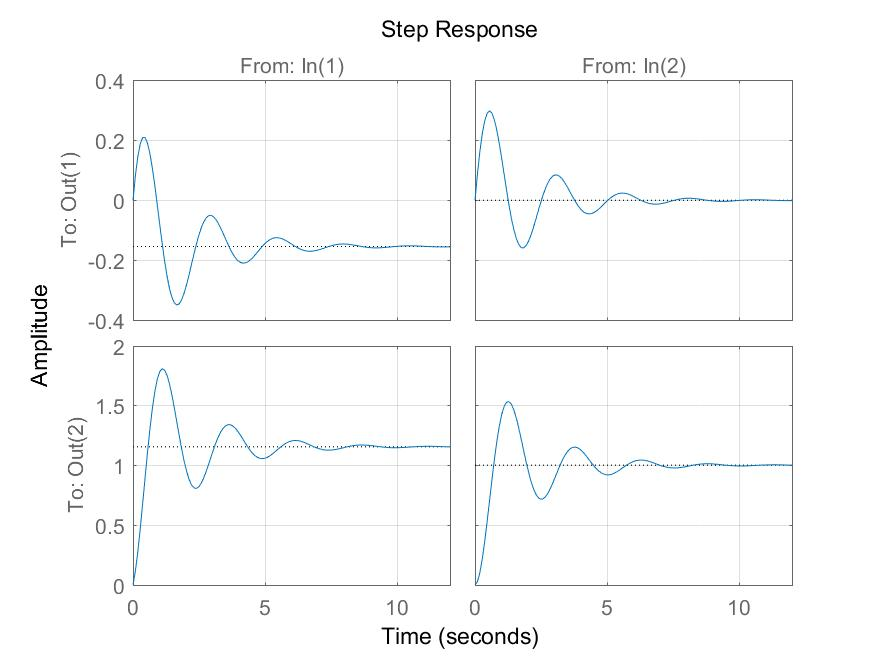
\includegraphics[width=8cm]  {fig/2-4.jpg}}      
 \caption{\label{1} 单位阶跃响应曲线} 
 \end{figure}
 
 \subsection{ 试验报告要求}
 \par 1.进行模型间的相互转换
 \par 2.试求以下系统
 \begin{equation}
    \dot x(t)\\=\begin{bmatrix}
    0 & -2 \\
    1 & -3 \\ \end{bmatrix}x(t)+ \begin{bmatrix}
    2\\
    0\\
    \end{bmatrix}u(t) ,  \quad      y(t)=\begin{bmatrix}
    1 & 0 \\\end{bmatrix}x(t) 
\end{equation}

 在阶跃输入信号和初始状态\[ x= \begin{bmatrix}1 & -1\end{bmatrix}^{T}\] \par 下的状态响应。编程实现,并给出响应曲线。

\par (1)阶跃输入信号下的状态响应,Matlab程序如下:
\par  \begin{lstlisting}[language=matlab,escapeinside=``]
A=[0 -2;1 -3];
B=[2;0];
C=[1 0];
D=0;
step(A,B,C,D)
grid on
\end{lstlisting}

\par 运行结果:
\newpage
\par \begin{figure}      
 \center{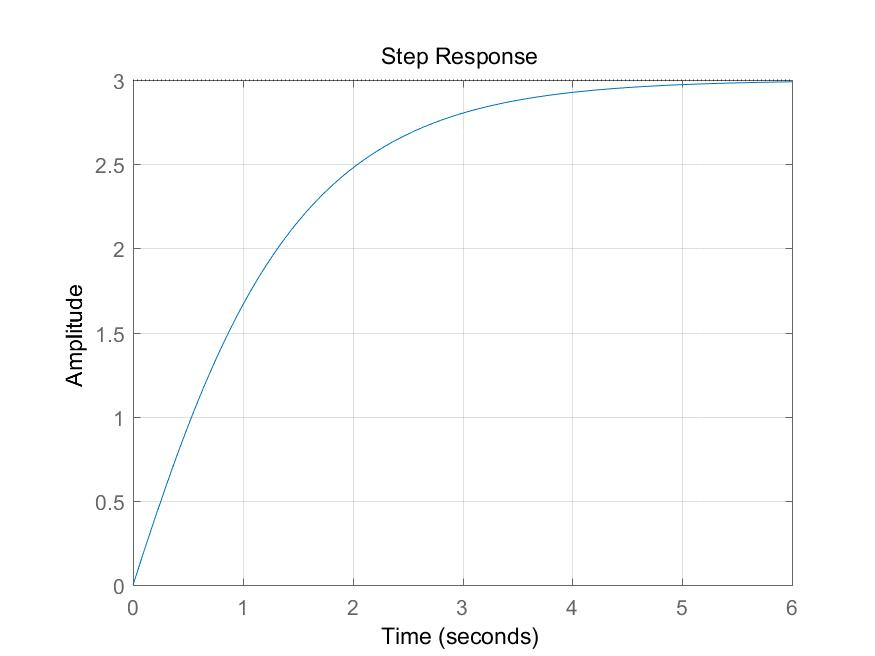
\includegraphics[width=8cm]  {fig/2-5.jpg}}      
 \caption{\label{1} 阶跃输入信号下的状态响应曲线} 
 \end{figure}

\par (2)初始状态\[ x= \begin{bmatrix}1 & -1\end{bmatrix}^{T}\] \par 下的状态响应,Matlab程序如下:
\par  \begin{lstlisting}[language=matlab,escapeinside=``]
A=[0 -2;1 -3];
B=[2;0];
D=0;
C=[1 0];
x0=[1;1];
[y,x,t]=initial(A,B,C,D,x0);
plot(t,x(:,1),t,x(:,2))
grid on
title('Response to Initial Condition')
xlabel('Time(sec)')
ylabel('x1,x2');
text(0.55,1.15,'x1')
text(0.4,-2.9,'x2')
\end{lstlisting}

\par 运行结果:
\newpage
\par \begin{figure}      
 \center{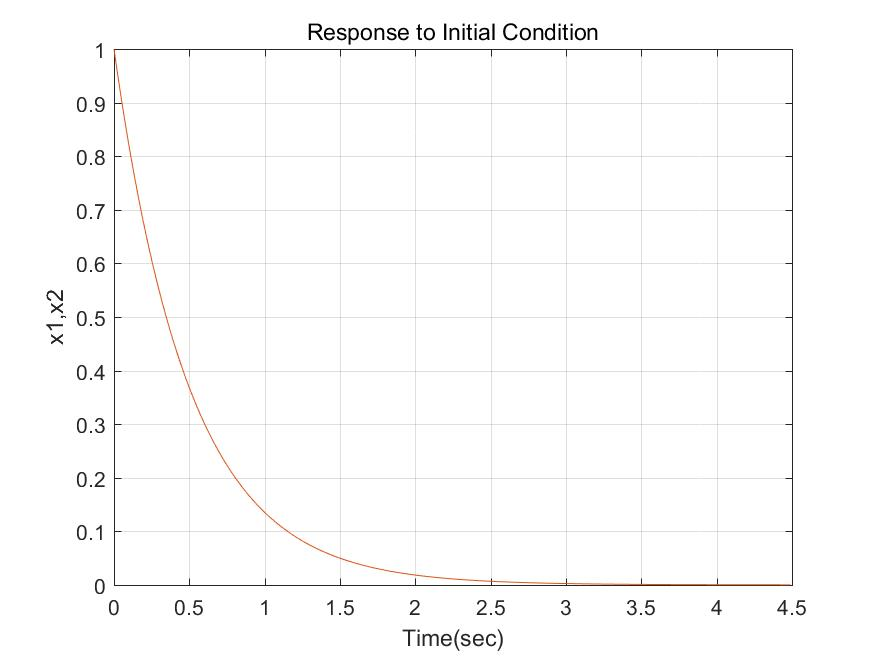
\includegraphics[width=8cm]  {fig/2-6.jpg}}      
 \caption{\label{1} 初始状态x下的状态响应曲线} 
 \end{figure}

\subsection{ 讨论}
\par  系统的状态轨迹和系统输入输出的关系。
\par  (1)在特定时刻t,状态矢量x(t)在状态空间中是一点。已知初始时刻t0的状态x(t0),就得到状态空间中的一个初始点。随着时间的推移,x(t)将在状态空间中描述出一条轨迹,称为状态迹线。
\par  (2)系统输入通过影响系统状态内部状态改变系统的状态轨迹,而内部状态也会影响外部输出。
		
		
\newpage
\section{实验三 \quad 系统能控性、能观性的判别}
\subsection{ 实验目的 }
\par 1.系统的能控性和能观测性的判别方法、系统的能控性和能观测性分解 
\par 2.了解 MATLAB 中相应的函数
\subsection{实验内容 }
\par 系统的模型表达式如下:		
\begin{equation}
    \dot x\\=\begin{bmatrix}
    0 & 1 \\
    -2 & -3 \\ \end{bmatrix}x+ \begin{bmatrix}
    0\\
    1\\
    \end{bmatrix}u ,  \quad      y=\begin{bmatrix}
    3 & 4 \\\end{bmatrix}x
\end{equation}
			
\par 1.判别系统的能控性		
\par Matlab程序如下:
\par  \begin{lstlisting}[language=matlab,escapeinside=``]		
A=[0 1;-2 -3];
B=[0;1];
Qc=ctrb(A,B);
n=rank(Qc);
L=length(A);
if n==L
    str='系统状态完全能控'
else 
    str='系统状态不完全能控'
end		
\end{lstlisting}		
		
\par 运行结果如下:		
\par  \begin{lstlisting}[language=matlab,escapeinside=``]		
str =
系统状态完全能控		
\end{lstlisting}			
		
\par 2.求系统的能控性分解后的模型		
\par Matlab程序如下:
\par  \begin{lstlisting}[language=matlab,escapeinside=``]			
A=[0 1;-2 -3];
B=[0;1];
C=[3 4];
[a,b,c,T,K]=ctrbf(  A,B,C)
sum(K)		
\end{lstlisting}			
		
\par 运行结果如下:		
\par  \begin{lstlisting}[language=matlab,escapeinside=``]		
a =
     0    -1
     2    -3
b =
     0
     1
c =
    -3     4
T =
    -1     0
     0     1
K =
     1     1
ans =
     2
\end{lstlisting}			
		
\subsection{实验内容 }
\par 调试完所有实验内容后,输入状态空间模型
\begin{equation}
    A=\begin{bmatrix}
    0 & 0 & -1\\
    1 & 0 & -3\\
    0 & 1 & -3\\ \end{bmatrix}  , \quad B=\begin{bmatrix}
   1\\
   1\\
   0\\ \end{bmatrix}   , \quad  C=\begin{bmatrix}
   0 & 1 & -2\\ \end{bmatrix}  , \quad D=0
\end{equation}

\par 1.判别系统的能观性
\par Matlab程序如下:
\par  \begin{lstlisting}[language=matlab,escapeinside=``]	
A=[0 0 -1;1 0 -3;0 1 -3];
B=[1;1;0];
C=[0 1 -2];
D=0;
Q0=obsv(A,C);
n=rank(Q0);
L=length(A);
if n==L
    str='系统状态完全能观'
else 
    str='系统状态不完全能观'
end
%%  实验要求2
[a,b,c,T,K]=obsvf(  A,B,C)
sum(K)
\end{lstlisting}	

\par 运行结果如下:		
\par  \begin{lstlisting}[language=matlab,escapeinside=``]	
str =
系统状态不完全能观
a =
   -1.0000    1.3416    3.8341
    0.0000   -0.4000   -0.7348
    0.0000    0.4899   -1.6000
b =
    1.2247
    0.5477
    0.4472
c =
         0   -0.0000    2.2361
T =
    0.4082    0.8165    0.4082
    0.9129   -0.3651   -0.1826
         0    0.4472   -0.8944
K =
     1     1     0
ans =
     2
\end{lstlisting}

\subsection{讨论}
\par 1.能控性和能观测性的定义。
\par (1)能控性的定义:
\par 线性连续定常系统:如果存在一个分段连续的输入u(t),能在有限时间区间[t$_{0}$,t$_{f}$]内,使系统由某一初始状态x(t$_{0}$),转移到指定的任一终端状态x(t$_{f}$),则称此状态是能控的。若系统的所有状态都是能控的,则称此系统是能控的。
\par 线性连续时变系统:其能控性的定义与定常系统的定义相同,但应强调强调在t$_{0}$时刻系统是能控的。
\par  离散时间系统:只考虑但输入的n阶线性定常离散系统:x(k+1)=Gx(k)+Hu(k),其中u(k)是标量控制作用,它在(k,k+1)区间内是个常值,其能控性定义为:若存在控制作用序列u(k),u(k+1),…,u(l-1)能将第k步的某个状态x(k)在第l步上到达零状态,即x(l)=0,其中l是大于k的有限数,那么就称此状态是能控的。若系统在第k步上的所有状态x(k)都是能控的,那么称此系统是状态完全能控的。
\par (2)能观测性的定义
\par 能观性所表示的是输出y(t)反映状态矢量x(t)的能力,与控制作用没有直接关系,所以分析能观性问题时,只需从齐次状态方程的输出方程出发。如果对任意给定的输入u,在有限观测时间t$_{f}$ 
$\geq$ $t_{0}$,使得根据[t$_{0}$,t$_{f}$]期间的输出y(t)能唯一地确定系统在初始时刻的状态x(t$_{0}$),则称状态x(t$_{0}$)是能观测的。若系统每个状态都是能观测的,则称系统是状态完全能观测的,或简称是能观的
\par 2.对于一个完全能控的系统,如何将其变换为能控标准型
\par (1)求出T$_{c1}$
\par (2)	通过公式\begin{equation}A =T_{c1}^{-1}AT_{c1}、b =T_{c1}^{-1}b,c =cT_{c1}\end{equation}求得A 、b 、c ,则得到系统的能控标准I型为:x=Ax+b u;y=cx


		
\newpage
\section{实验四 \quad 系统稳定性仿真实验}
\subsection{ 实验目的 }
\par 1.掌握线性系统稳定性的判别方法
\par 2.了解 MATLAB 中相应的函数 
\subsection{实验内容 }
\par 判定如下系统的李亚普诺夫稳定性,系统的模型表达式如下:		
\begin{equation}
    \dot x\\=\begin{bmatrix}
    0 & 1 \\
    -1 & -1 \\ \end{bmatrix}x
\end{equation}		
		
\par Matlab程序如下:
\par  \begin{lstlisting}[language=matlab,escapeinside=``]	
A=[0 1;-1 -1];
Q=eye(size(A,1));
P=lyap(A,Q);
P_eig=eig(P);
if min(P_eig)>0
    disp('The system is Lypunov stable.')
else 
    disp('The system is not Lypunov stable.')
end
\end{lstlisting}
\par 运行结果如下:		
\par  \begin{lstlisting}[language=matlab,escapeinside=``]			
	The system is Lypunov stable.	
\end{lstlisting}		
		
\subsection{试验报告要求}
\par 输入状态空间模型如下:	
\begin{equation}
    A=\begin{bmatrix}
    -3 & -8 & -2 & -4\\
    1 & 0 & 0 & 0\\
    0 & 1 & 0 & 0\\
    0 & 0 & 1 & 0\\ \end{bmatrix}  , \quad B=\begin{bmatrix}
   0\\
   0\\
   1\\
   1\\ \end{bmatrix}   , \quad  C=\begin{bmatrix}
   0 & 0 & 1 & 1\\ \end{bmatrix}  , \quad D=0
\end{equation}	
	
\par 判定如下系统的李亚普诺夫稳定性。
\par Matlab程序如下:
\par  \begin{lstlisting}[language=matlab,escapeinside=``]	
A=[-3 -8 -2 -4;1 0 0 0;0 1 0 0;0 0 1 0];
Q=eye(size(A,1));
P=lyap(A,Q);
P_eig=eig(P);
if min(P_eig)>0
    disp('The system is Lypunov stable.')
else 
    disp('The system is not Lypunov stable.')
end
\end{lstlisting}
\par 运行结果如下:		
\par  \begin{lstlisting}[language=matlab,escapeinside=``]			
	The system is Lypunov stable.	
\end{lstlisting}		
	
\subsection{讨论}	
\par 系统稳定性的含义。	
\par  (1)从经典控制理论可知,线性系统的稳定性只取决于系统的结构和参数而与系统的初始条件及外界扰动的大小无关。但非线性系统的稳定性则还与初始条件及外界扰动的大小有关。因此在经典控制理论中没有给出稳定性的一般定义。
\par  (2)李雅普诺夫给出了对任何系统都普遍适用的稳定性的一般定义。即系统响应的幅值是有界的,则称平衡状态x$_{e}$为李雅普诺夫意义下稳定,简称稳定。
	
	
\newpage
\section{实验五 \quad 状态反馈及状态观测器的设计}
\subsection{ 实验目的 }
\par 1.熟悉状态反馈矩阵的求法
\par 2.熟悉状态观测器设计方法
\subsection{实验内容 }
\par 某控制系统的状态方程描述如下:	
\begin{equation}
    A=\begin{bmatrix}
    -10 & -35 & -50 & -24\\
    1 & 0 & 0 & 0\\
    0 & 1 & 0 & 0\\
    0 & 0 & 1 & 0\\ \end{bmatrix}  , \quad B=\begin{bmatrix}
   1\\
   0\\
   0\\
   0\\ \end{bmatrix}   , \quad  C=\begin{bmatrix}
   1 & 7 & 24 & 24\\ \end{bmatrix}
\end{equation}		
\par 通过状态反馈使系统的闭环极点配置在\[P=\begin{bmatrix}-30 & -1.2 & -2.4 \pm 4i \end{bmatrix}\]置上,求出状态 反馈阵 K,并绘制出配置后系统的时间响应曲线。
\par 要求:
\par  (1)求出系统的状态空间模型
\par  (2)依据系统动态性能的要求, 确定所希望的闭环极点 P
\par  (3)利用上面的极点配置算法求系统的状态反馈矩阵 K
\par  (4)检验配置后的系统性能
\par Matlab程序如下:		
\par  \begin{lstlisting}[language=matlab,escapeinside=``]			
A=[-10 -35 -50 -24;1 0 0 0;0 1 0 0;0 0 1 0];
B=[1;0;0;0];
C=[1 7 24 24];
D=0;
disp('原系统的极点为:');
p=eig(A)'
P=[-30;-1.2;-2.4+sqrt(-16);-2.4-sqrt(-16)];
disp('状态反馈向量为');
K=place(A,B,P)
disp('配置后的系统极点为:')
p=eig(A-B*K)'
disp('配置后的系统矩阵为:')
sys=ss(A-B*K,B,C,D)
step(sys/dcgain(sys))
grid on
\end{lstlisting}		
\par 运行结果如下:		
\par  \begin{lstlisting}[language=matlab,escapeinside=``]			
原系统的极点为:
p =
   -4.0000   -3.0000   -2.0000   -1.0000
状态反馈向量为
K =
   26.0000  172.5200  801.7120  759.3600
配置后的系统极点为:
p =
  1 至 3 列
 -30.0000 + 0.0000i  -2.4000 - 4.0000i  -2.4000 + 4.0000i
  4 列
  -1.2000 + 0.0000i
配置后的系统矩阵为:
sys =
  A = 
           x1      x2      x3      x4
   x1     -36  -207.5  -851.7  -783.4
   x2       1       0       0       0
   x3       0       1       0       0
   x4       0       0       1       0
  B = 
       u1
   x1   1
   x2   0
   x3   0
   x4   0
  C = 
       x1  x2  x3  x4
   y1   1   7  24  24
  D = 
       u1
   y1   0
\end{lstlisting}		
\par 响应曲线如下:
\newpage	
\par \begin{figure}      
 \center{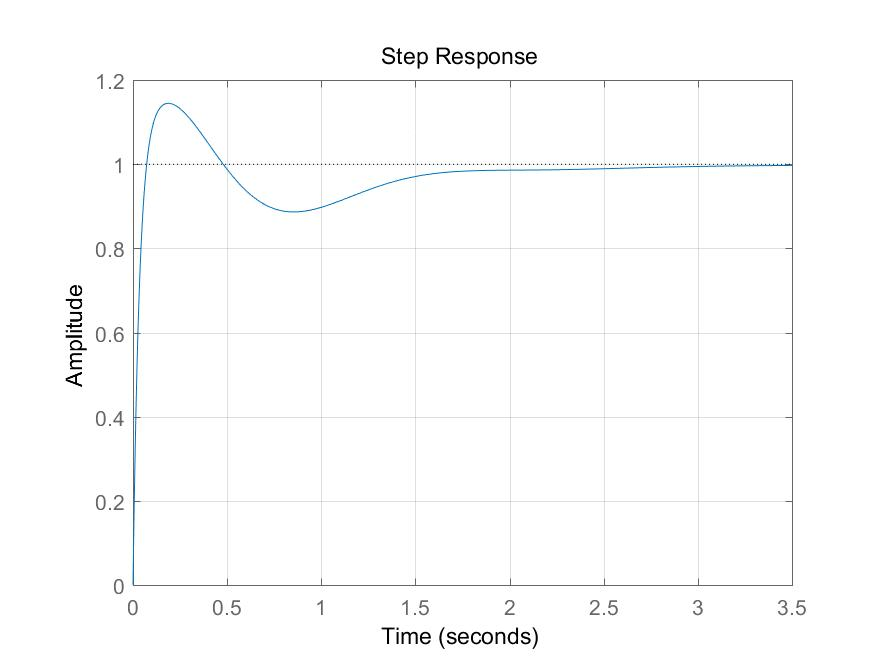
\includegraphics[width=8cm]  {fig/5-1.jpg}}      
 \caption{\label{1} 极点配置后系统的时间响应曲线} 
 \end{figure}	
	
\subsection{实验总结与心得}	
\par  	通过这次实验,我熟悉状态反馈矩阵的求法,同时了解了状态观测器设计方法。通过用matlab仿真系统的闭环极点配置,加深理解理论知识,同时扩展自己的知识面,提高自己的技能。	
\end{document}